\section{Testen}

\subsection{Funktionstest}

\subsubsection{Webapplikation}

Um die Webapplikation zu testen wurde ein Funktionstest durchgeführt. Dieser umfasst die in Kapitel \ref{sec:funkAnforderungenAnwender} festgesetzten Anforderungen und ist im Folgenden bebildert beschrieben.\newline





\begin{wrapfigure}[8]{l}{0.4\textwidth}
 \centering
 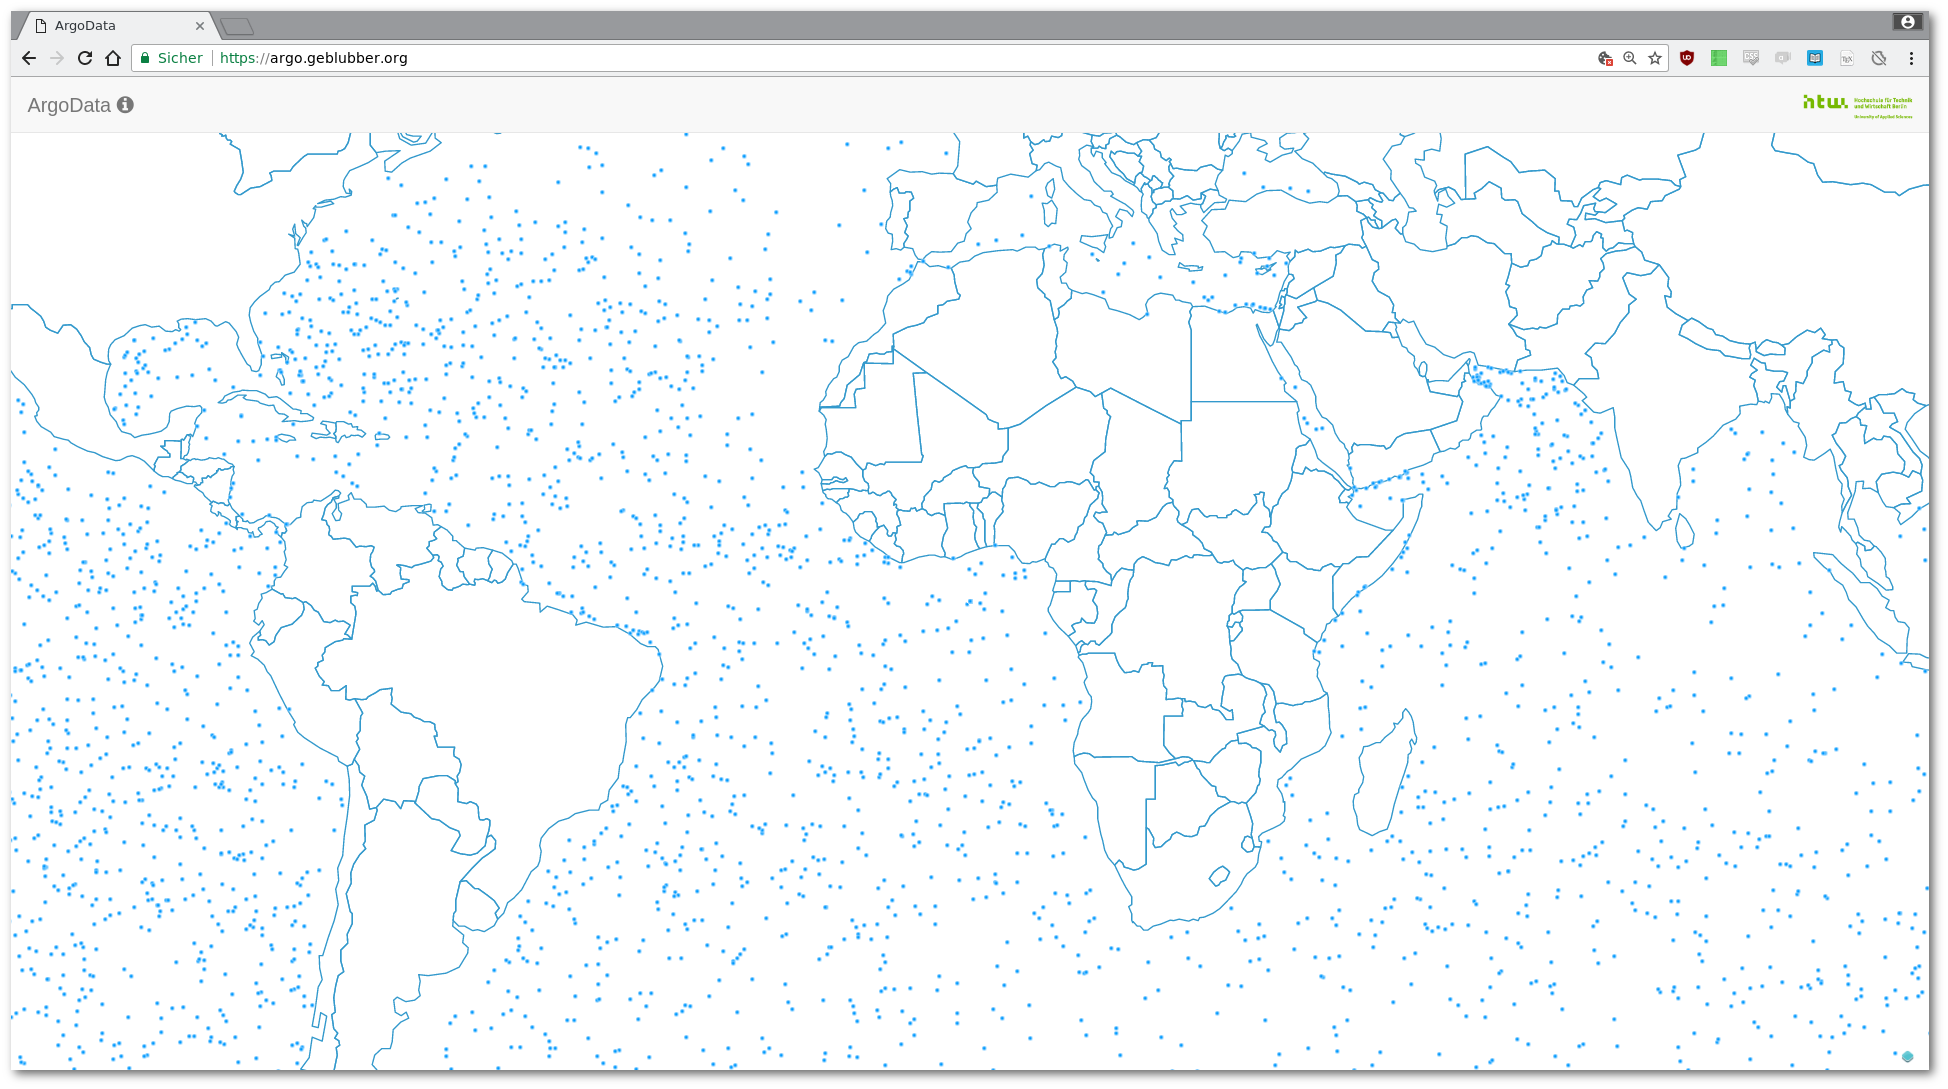
\includegraphics[width=0.39\textwidth]{pix/ftest/001.png}

 \caption{\textbf{Funktionstest I} Der Aufruf der Webapplikation}
 \label{fig:ftest001}
\end{wrapfigure}  


Wird die Webpräsenz ArgoData unter ihr zugewiesenen URL aufgerufen, werden die Grenzen der Ozeane und Kontinente über eine Weltkarte dargestellt. Die Karte ist über eine Vektorrepräsentation dargestellt, Landmarker wie Straßen und Städte sind daruf nicht zu erkennen. Die letzte Position der Messstationen ist über die jeweilige Position auf der Karte ersichtlich.
\newline\newline\newline


\begin{wrapfigure}[10]{l}{0.4\textwidth}
 \centering
 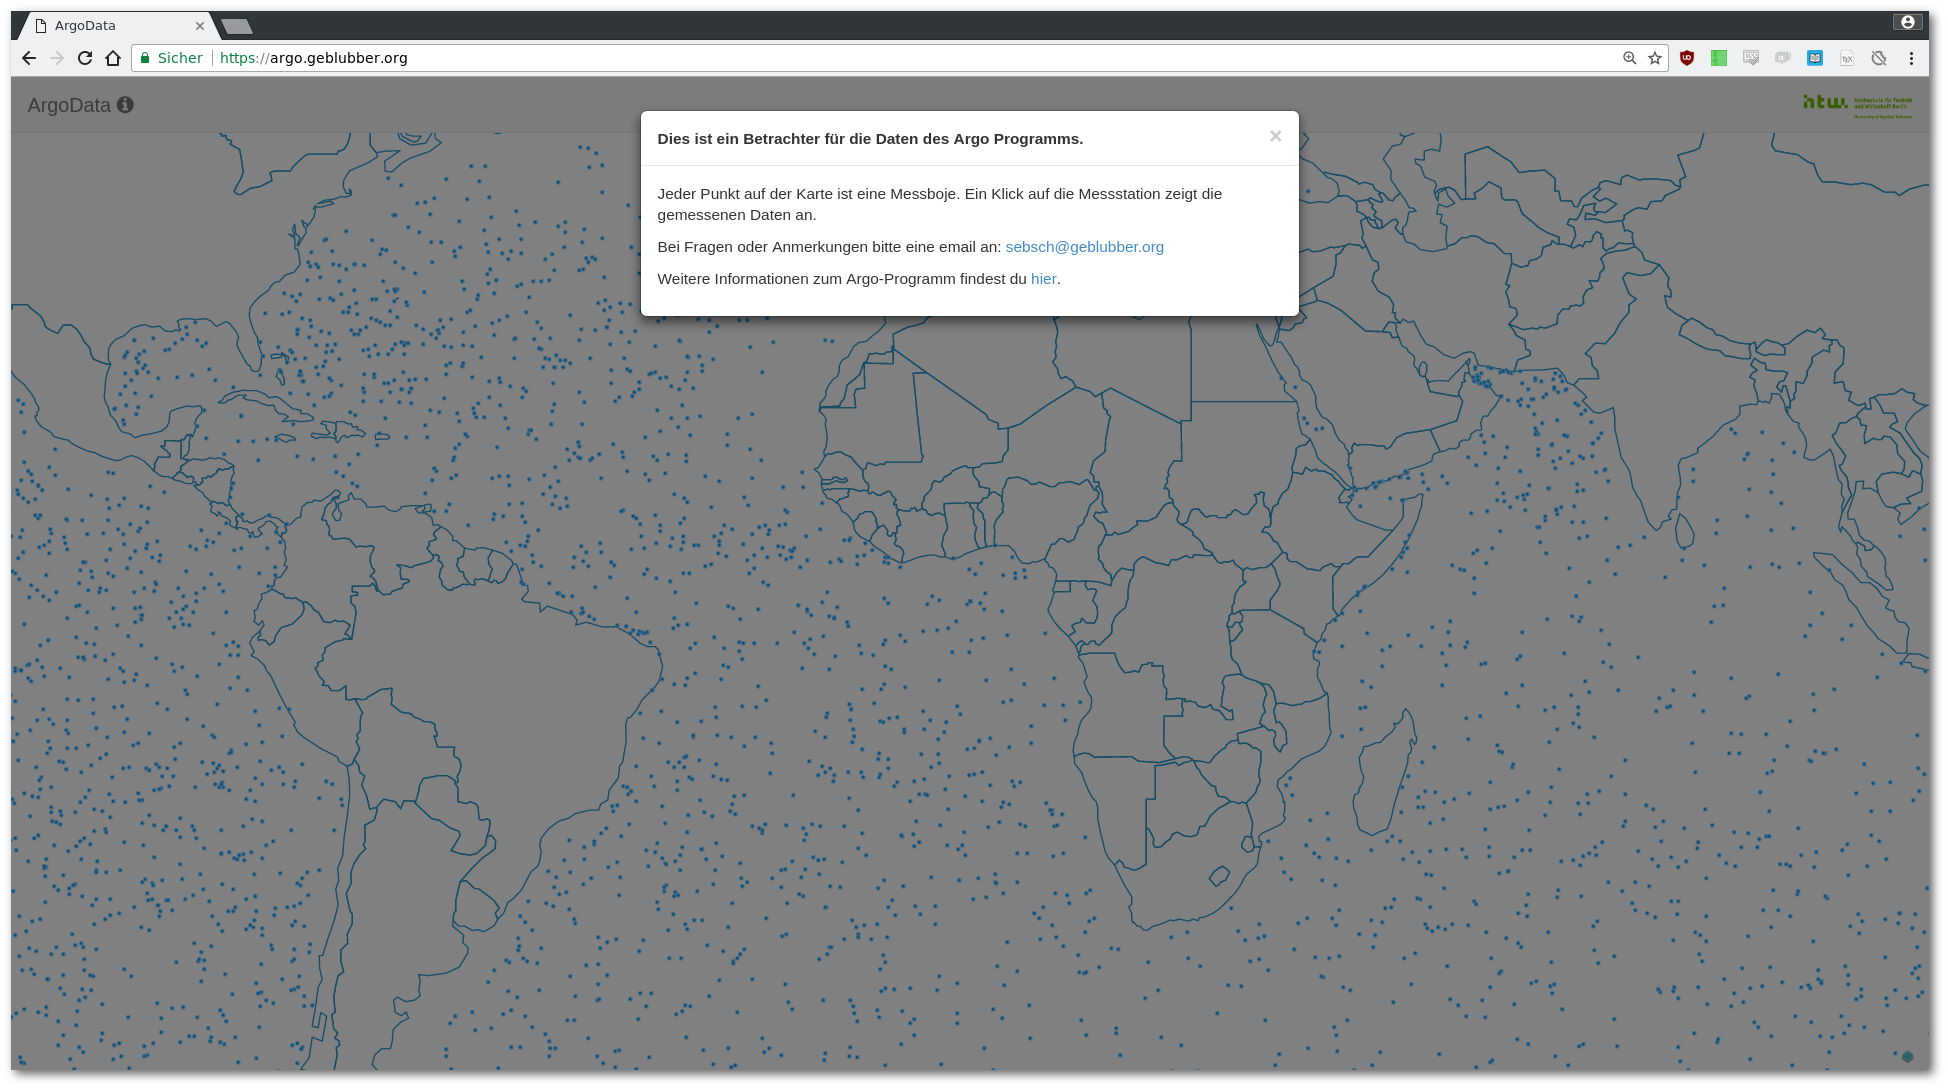
\includegraphics[width=0.39\textwidth]{pix/ftest/001b.png}

 \caption{\textbf{Funktionstest II} Die Anzeige der Hilfe}
 \label{fig:ftest001b}
\end{wrapfigure} 

Durch Anklicken des Infobuttons erhält der Benutzer über ein modal eine Kurzhilfe angezeigt. Diese erklärt die Grundlegende Funktion der Webseite, stellt Kontaktdaten bereit und stellt über einen Weblink eine Verbindung zum Argo-Programm her.
\newline\newline\newline\newline


\begin{wrapfigure}[10]{l}{0.4\textwidth}
 \centering
 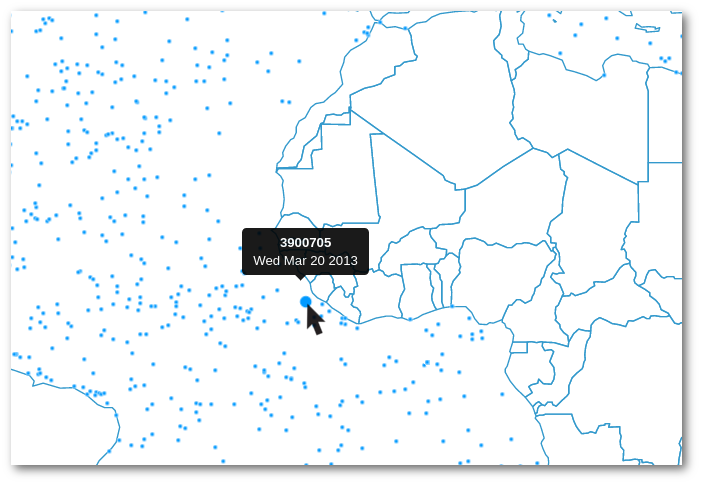
\includegraphics[width=0.39\textwidth]{pix/ftest/002.png}

 \caption{\textbf{Funktionstest III} Mousehover über Messstation}
 \label{fig:ftest002}
\end{wrapfigure} 

Wird der Mauszeiger über die Repräsentation einer Messstation geführt, so erscheinen Grundlegende Daten der Argo-Boje. Dies umfasst den eindeutigen Identifier sowie das Datum des letzten Messvorgangs. 
\newline\newline\newline\newline\newline


\begin{wrapfigure}[10]{l}{0.4\textwidth}
 \centering
 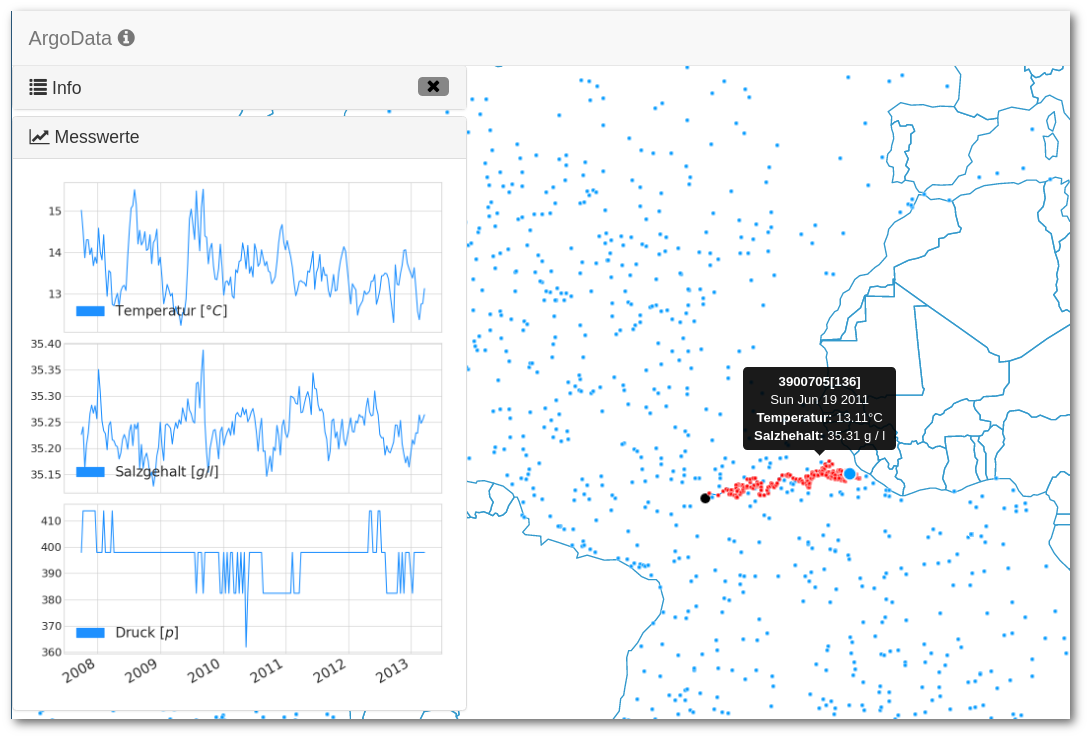
\includegraphics[width=0.39\textwidth]{pix/ftest/003.png}

 \caption{\textbf{Funktionstest IV} Werte werden Angezeigt}
 \label{fig:ftest003}
\end{wrapfigure}

Durch einen Mausklick auf die Kartendarstellung der Argo-Boje werden weiterführende Daten angefordert. Die Messwerte werden über Funktionsplots an der linken Seite der Webseite dargestellt. Dabei sind über die X-Achse der zeitliche Verlauf und über die Y-Achse der jeweilige Messwert kodiert. Die gemessenen Werte umfassen dabei Temperatur, Salzgehalt sowie dem Druck.  Der Ort der Messwerterhebung wird durch einen Punkt auf der Karte repräsentiert. Wird der Mauszeiger über diese Repräsentation geführt, werden neben dem Datum der Messung auch die gemessenen Werte dargestellt.


\begin{wrapfigure}[10]{l}{0.4\textwidth}
 \centering
 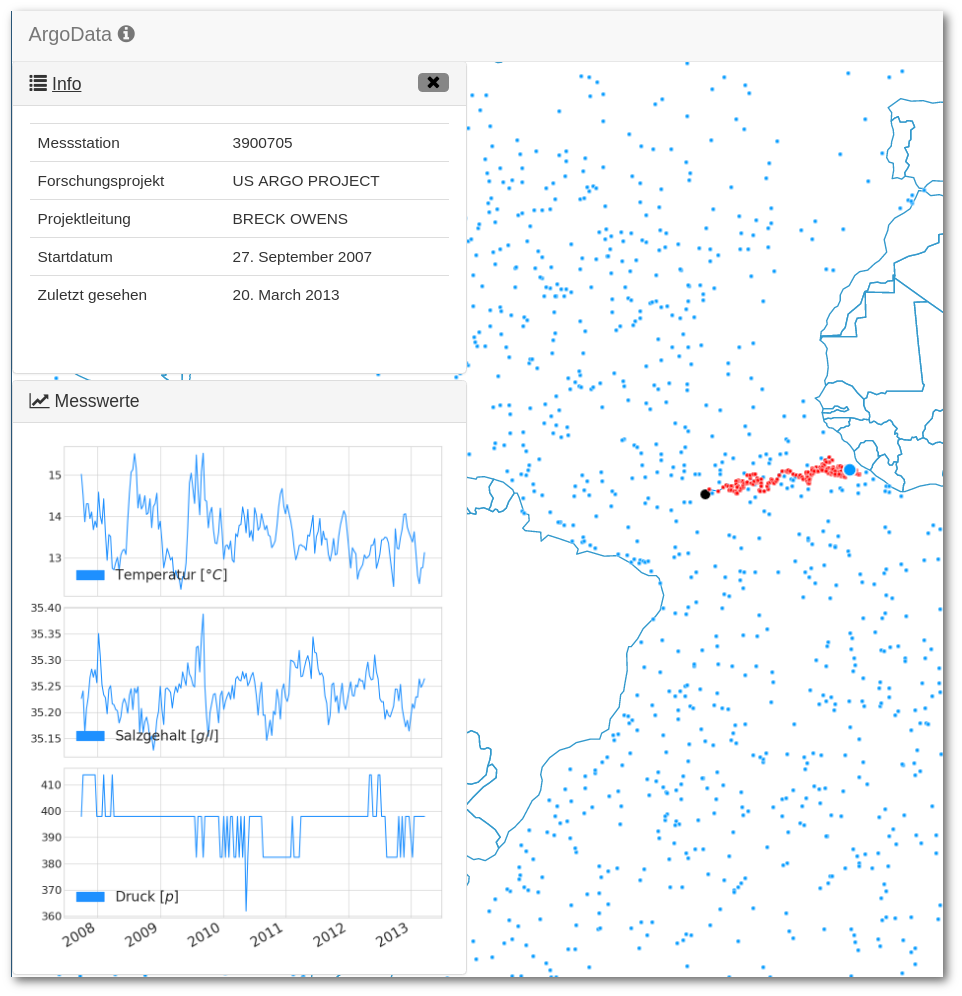
\includegraphics[width=0.35\textwidth]{pix/ftest/003b.png}

 \caption{\textbf{Funktionstest V} Metainformationen werden angezeigt}
 \label{fig:ftest003b}
\end{wrapfigure}

Wird der Reiter Info angeklickt, so werden weitere Informationen zur Messstation sichtbar. Diese Umfassen den Identifier der Messstation, das verantwortliche Forschungsprojekt, den Besitzer der Boje sowie das Startdatum und das Datum der letzten Messung.
\newline\newline\newline\newline
\newline\newline\newline


\begin{wrapfigure}[10]{l}{0.4\textwidth}
 \centering
 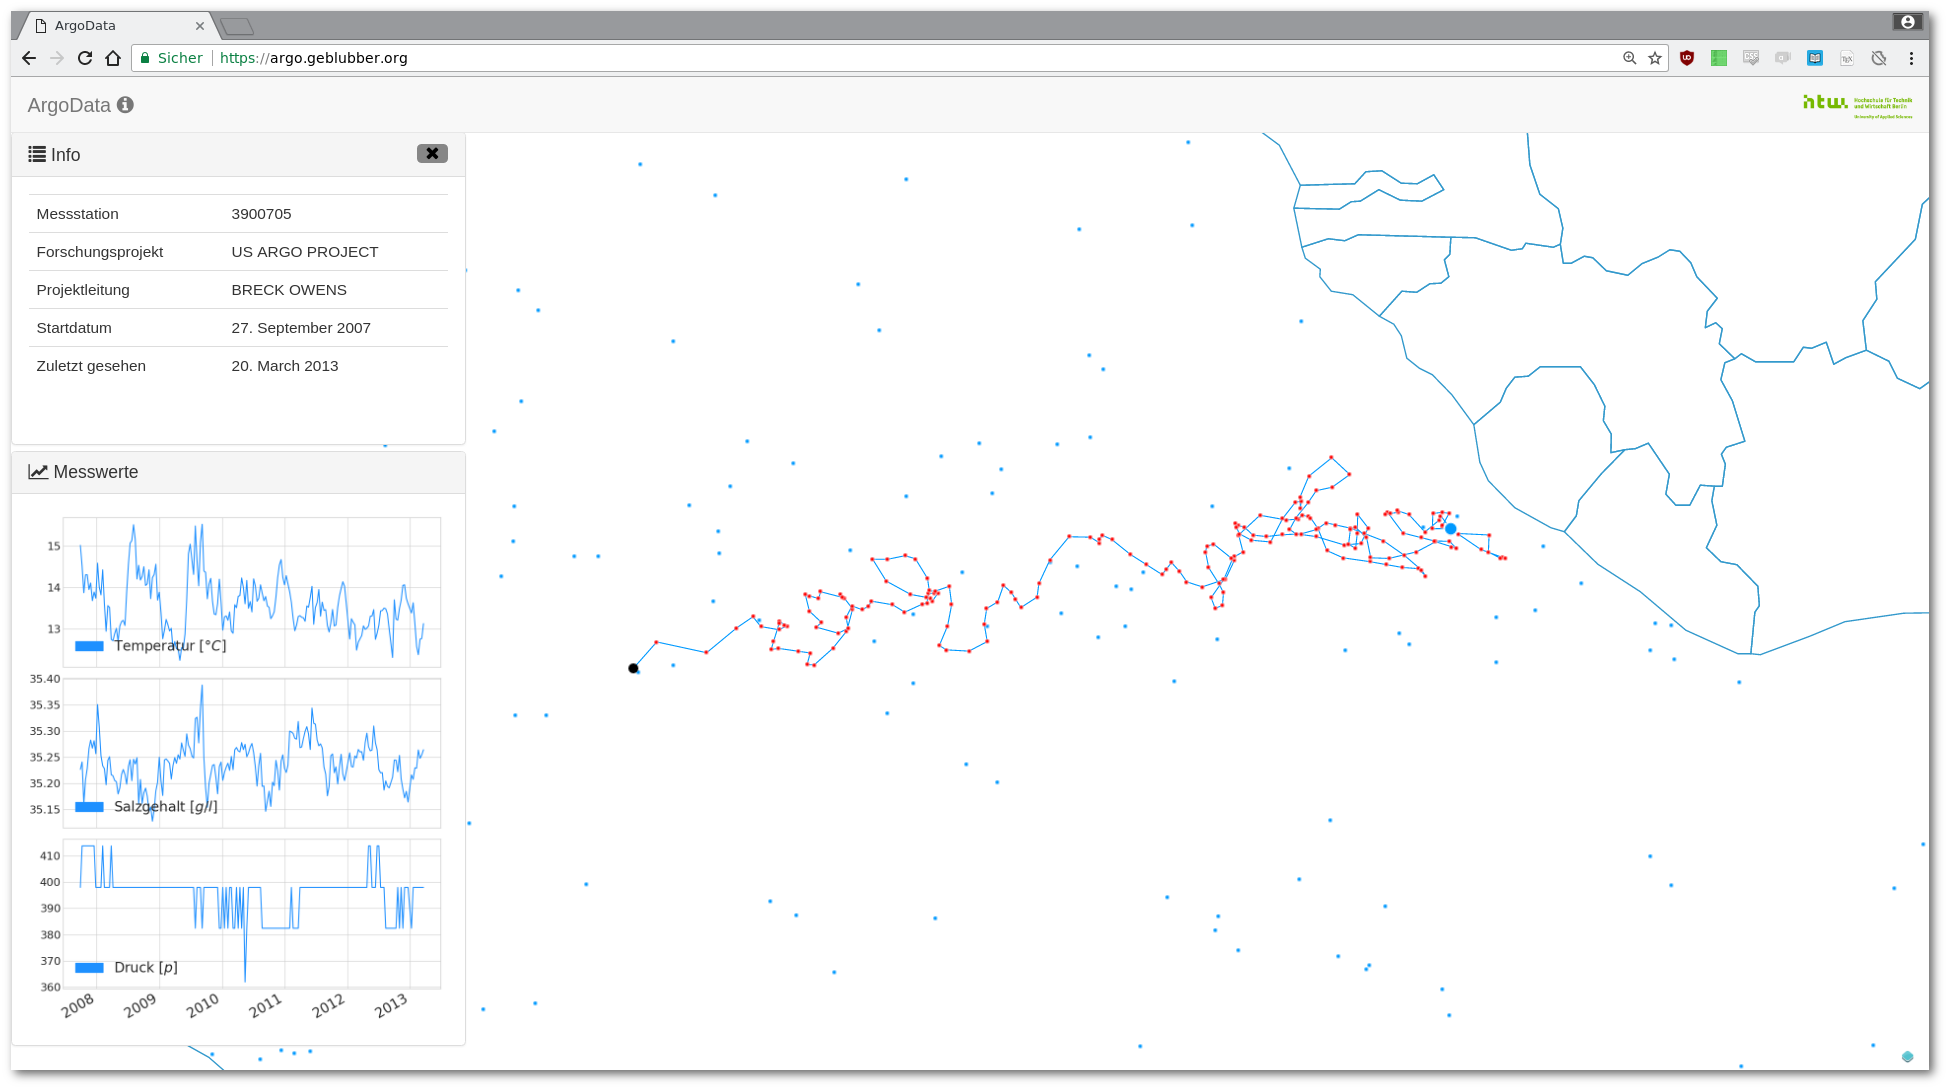
\includegraphics[width=0.35\textwidth]{pix/ftest/004.png}

 \caption{\textbf{Funktionstest VI} Der Pfad der Messstatioon kann zurückverfolgt werden}
 \label{fig:ftest004}
\end{wrapfigure}

Zwischen zwei Messpunkten wird der zurückgelegte Weg über eine Linie dargestellt. Somit kann der Weg den eine Messstation zurückgelegt hat, um die Daten zu erheben klar nachvollzogen werden.
\newline\newline\newline\newline
\newline\newline\newline


\begin{wrapfigure}[10]{l}{0.4\textwidth}
 \centering
 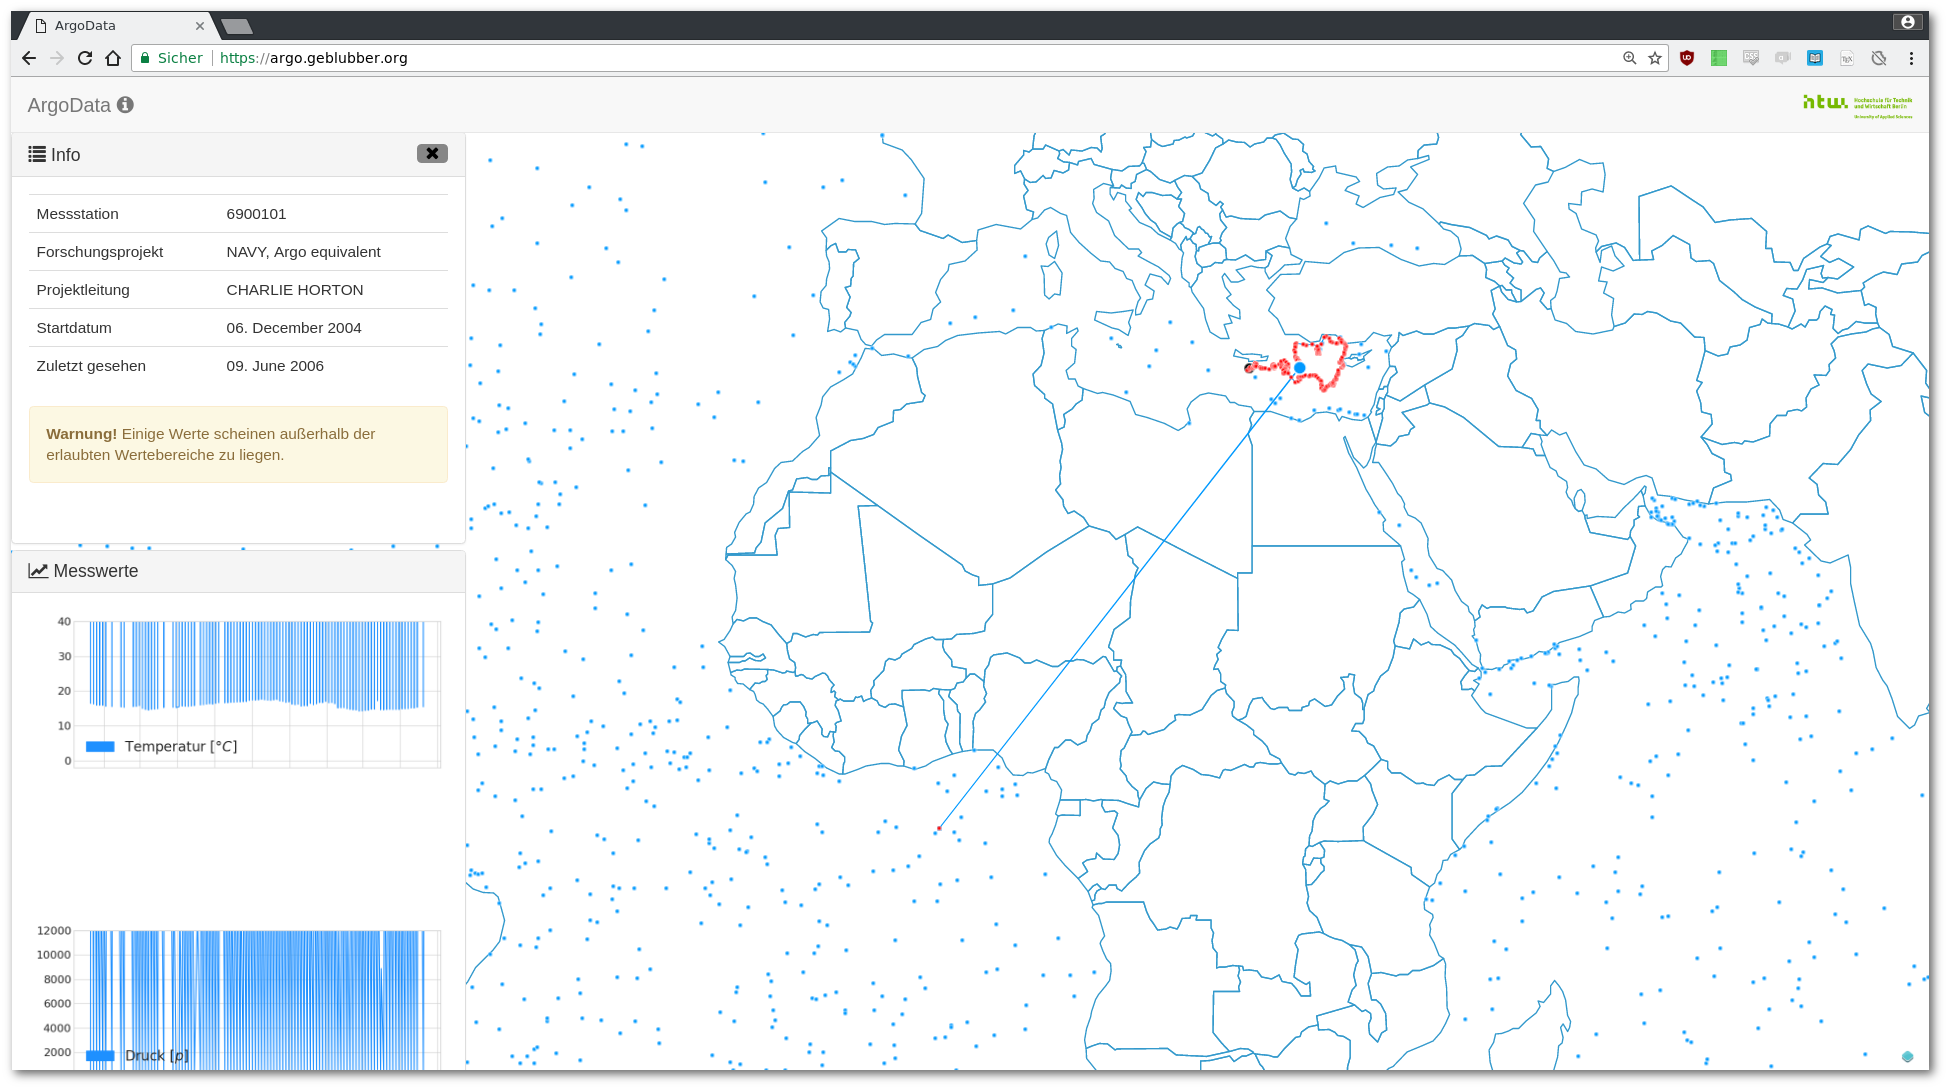
\includegraphics[width=0.35\textwidth]{pix/ftest/00fail.png}

 \caption{\textbf{Funktionstest VI} Fehlerhafte Daten werden markiert}
 \label{fig:ftest00fail}
\end{wrapfigure}

Fehlerhafte Daten werden durch eine Markierung hervorgehoben. Dafür wird eine Warnung ausgegeben, die den Benutzer informiert, dass die Daten, die gerade angezeigt werden, zum Teil die Wertebereiche überschritten haben. Die Achsen der Funktionsplots werden auf die Wertebereiche beschränkt und Plots von mit nan kodierten Messwerten nicht dargestellt.
\newline
\newline



\subsubsection{Aggregation der Daten}

In Listing \ref{lst:renewdatash} ist der Prozess der Datenerneuerung zu sehen. Dieser Umfasst die in Kapitel \ref{sec:funkAnforderungenAdmin} festgelegten Anforderungen. Der Ablauf ist im Folgenden beschrieben.

\begin{python}[%
        label={lst:renewdatash},%
        caption={Erneuerung des Datensatzes}]
 -> # bash /root/argo_proto/renew_data.sh
(!) Starting renew process at Tue Mar  6 12:41:24 CET 2018.
 >> Downloading new data...
        done.
Datafolder: /root/aoml/
||||||||||||||||||||||||||||||||||| 6711/6711 [2:02:33<00:00,  1.10s/it]
 >> Dumping tmpdb to /tmp/argo_db.sql ...
        done. [164601410 Mar  6 14:44 /tmp/argo_db.sql]
 >> Renew production database ...
        done.
 >> Renew Argos cache...  
        done.

Process finished.
This took  7381 seconds.
We had a downtime of 11 seconds.
So long and thanks for all the fish. Bye.
\end{python}

\begin{description}
 \item [Daten herunterladen] 
    Die Daten des Argo-Programms werden heruntergeladen. Es handelt sich um die Livedaten nach der Qualitätskontrolle aus der Quelle \texttt{aoml}. Für das herunterladen wird rsync verwendet. In der Quelle nicht mehr vorhandene Daten werden gelöscht.
    
    
 \item [Daten aggregieren]
    Der Aggregationsteil der hier entwickelten Software wird verwendet, die soeben erneuerten Daten in die Datenbank zu überführen. Um Ausfallzeiten der Webapplikation möglichst gering zu halten, werden die Daten zunächst in deine Temporäte Datenbank geschrieben. Über einen Ladebalken wird der derzeitige Stand dieses Prozesses sichtbar. Es ist außerdem ersichtlich, dass die Daten von 6711 Messstationen in 2 Stunden, 2 Minuten und 30 Sekunden in die Datenbank überführt wurden.
    
 \item [Erstellen eines Datenbankdumps]
    Um die daten in die Produktionsdatenbank zu überführen, werden die Tabellen der temporären Datenabnk gedumpt. Es ist ersichtlich, dass der Dump eine Größe von  164601410 byte (ca. 20 Megabyte) umfasst.
    
 \item [Einspielen des Datenbankdumps]
    Über die Funktionalitäten des Postgresql-Clients \texttt{psql} werden die Daten in die Produktionsdatenbank überführt. Dieser Prozess erfordert eine Ausallzeit der Webapplikation von 11 Sekunden. 
    
 \item [Erneuern des Caches zur Anzeige der Argo-Floats]
    Um die Daten in der Anzeige zu erneuern, wird der Cache neu geschrieben. Für diesen Zweck wird ein GET-Request an die hierfür festgelegte URL gesendet. Die Webapplikation erneuert daraufhin den Cache. Und die Webapplikation ist mit den neuen daten einsatzbereit.
\end{description}



\newpage
\subsection{Usability-Umfrage}
